\documentclass{standalone}
\usepackage{times}
\usepackage{mathtools}

\usepackage{tikz}
\usetikzlibrary{positioning,fit,shapes,calc,decorations.pathreplacing}
\usetikzlibrary{backgrounds}
\usetikzlibrary{arrows.meta}
\usetikzlibrary{shapes,snakes}

\definecolor{processblue}{cmyk}{1,1,1,0}
\definecolor{accent}{rgb}{0.6,0.6,0.6}
\definecolor{accent2}{rgb}{0.9,0.9,0.9}

\begin{document}
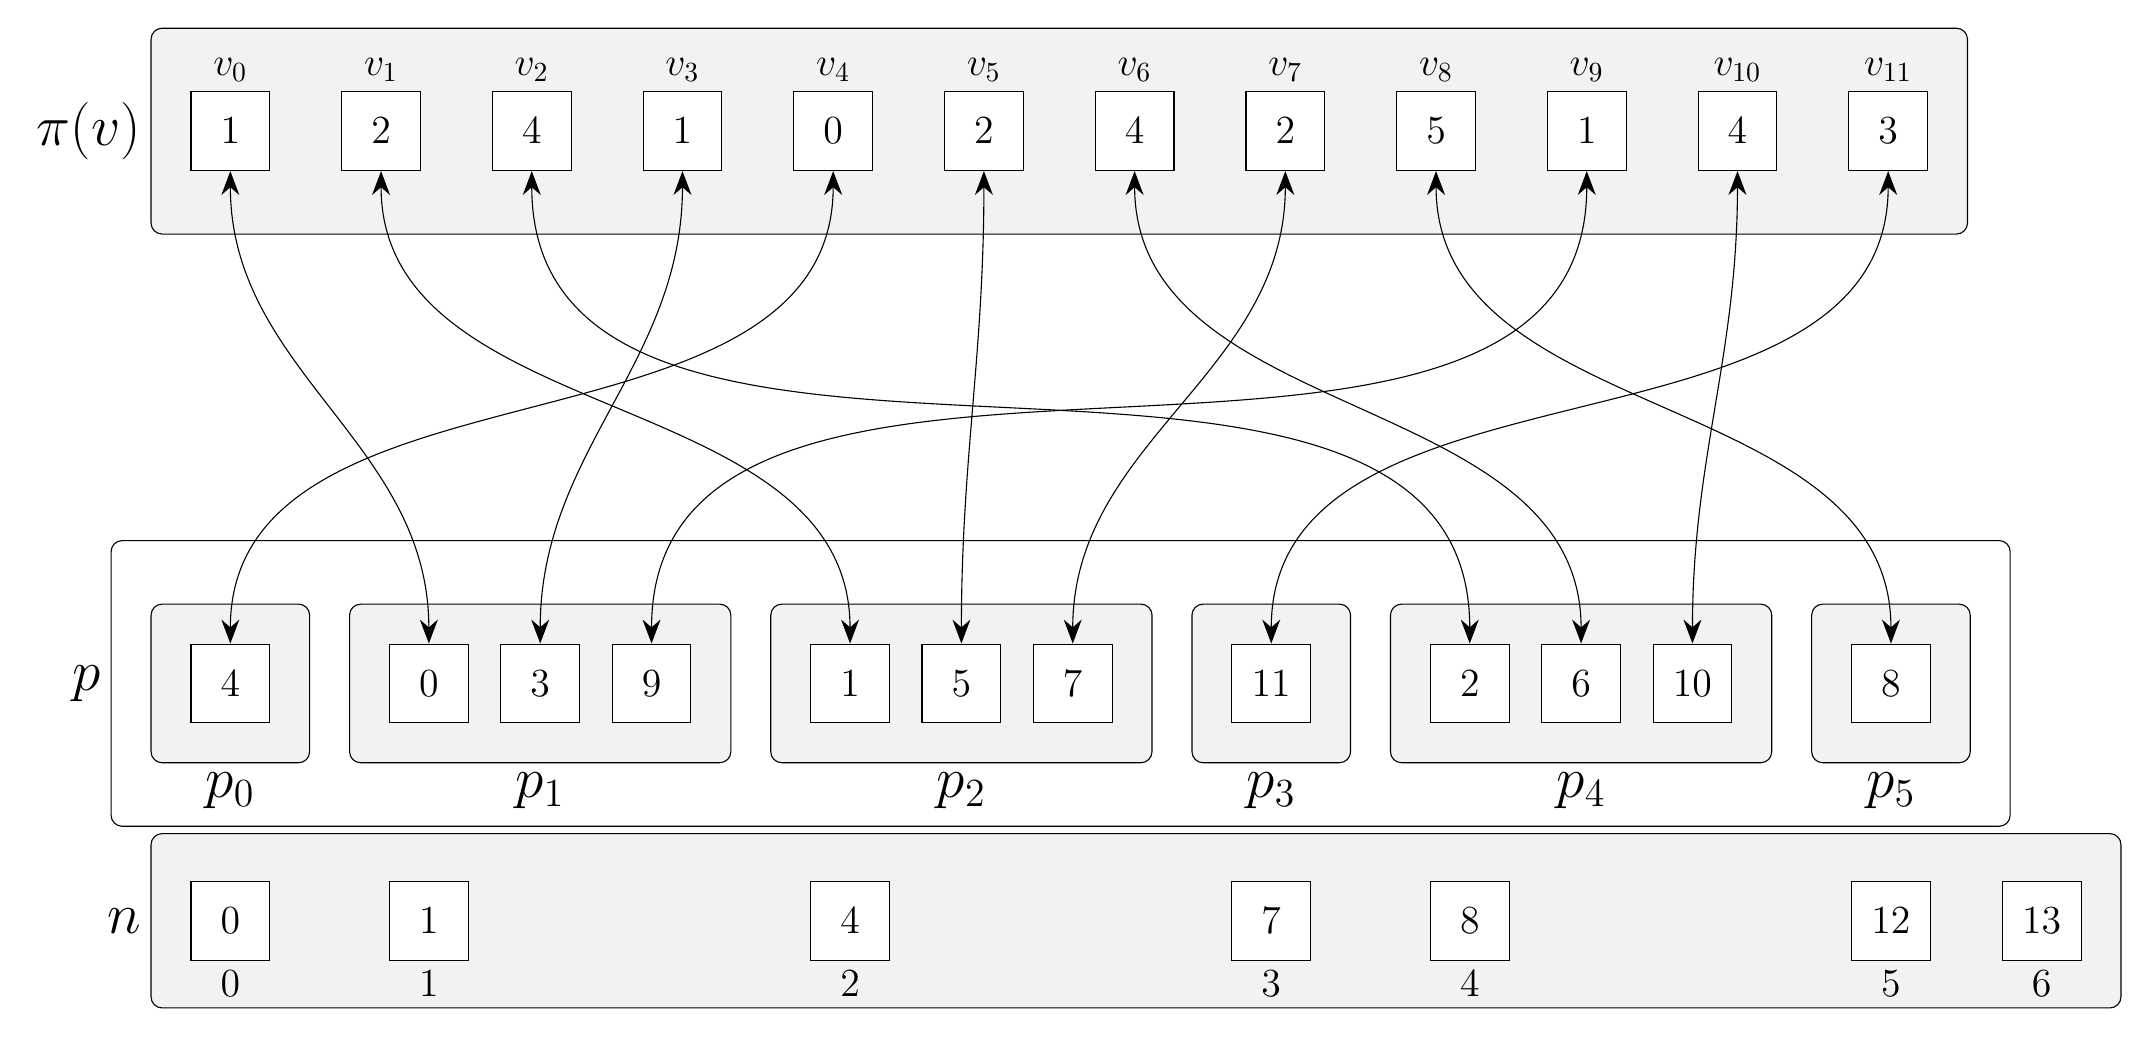
\begin{tikzpicture}[
  data/.style = {
    draw,
    rectangle,
    fill = white,
    minimum width = 1.0cm,
    minimum height = 1.0cm,
  },
  next/.style = {
    draw,
    circle,
    fill=black,
  },
  edge/.style = {
    draw,
    rectangle,
    rounded corners,
    minimum width = 0.5cm,
    minimum height = 0.5cm,
  },
  vedge/.style = {
    edge,
    top color = black!5,
    bottom color = black!5,
  },
  fedge/.style = {
    edge,
    top color = accent,
    bottom color = accent,
  },
  >={Stealth[scale=1.8]},
]

  % \clip (-3.5,-3.0) rectangle (18,2.5);

  \node[data,label={\Large $v_{0}$}] (v0) {\Large $1$};
  \node[data,label={\Large $v_{1}$}] (v1) [right=0.9cm of v0] {\Large $2$};
  \node[data,label={\Large $v_{2}$}] (v2) [right=0.9cm of v1] {\Large $4$};
  \node[data,label={\Large $v_{3}$}] (v3) [right=0.9cm of v2] {\Large $1$};
  \node[data,label={\Large $v_{4}$}] (v4) [right=0.9cm of v3] {\Large $0$};
  \node[data,label={\Large $v_{5}$}] (v5) [right=0.9cm of v4] {\Large $2$};
  \node[data,label={\Large $v_{6}$}] (v6) [right=0.9cm of v5] {\Large $4$};
  \node[data,label={\Large $v_{7}$}] (v7) [right=0.9cm of v6] {\Large $2$};
  \node[data,label={\Large $v_{8}$}] (v8) [right=0.9cm of v7] {\Large $5$};
  \node[data,label={\Large $v_{9}$}] (v9) [right=0.9cm of v8] {\Large $1$};
  \node[data,label={\Large $v_{10}$}] (v10) [right=0.9cm of v9] {\Large $4$};
  \node[data,label={\Large $v_{11}$}] (v11) [right=0.9cm of v10] {\Large $3$};

  \node[data] (p00) [below=6cm of v0] {\Large $4$};
  \begin{scope}[on background layer]
    \node[vedge,fit=(p00) (p00),inner sep=0.5cm,label={below: \huge $p_0$}] (p0) {};
  \end{scope}

  \node[data] (p10) [right=1.0cm of p0] {\Large $0$};
  \node[data] (p11) [right=0.4cm of p10] {\Large $3$};
  \node[data] (p12) [right=0.4cm of p11] {\Large $9$};
  \begin{scope}[on background layer]
    \node[vedge,fit=(p10) (p12),inner sep=0.5cm,label={below: \huge $p_1$}] (p1) {};
  \end{scope}

  \node[data] (p20) [right=1.0cm of p1] {\Large $1$};
  \node[data] (p21) [right=0.4cm of p20] {\Large $5$};
  \node[data] (p22) [right=0.4cm of p21] {\Large $7$};
  \begin{scope}[on background layer]
    \node[vedge,fit=(p20) (p22),inner sep=0.5cm,label={below: \huge $p_2$}] (p2) {};
  \end{scope}

  \node[data] (p30) [right=1.0cm of p2] {\Large ${11}$};
  \begin{scope}[on background layer]
    \node[vedge,fit=(p30) (p30),inner sep=0.5cm,label={below: \huge $p_3$}] (p3) {};
  \end{scope}

  \node[data] (p40) [right=1.0cm of p3] {\Large $2$};
  \node[data] (p41) [right=0.4cm of p40] {\Large $6$};
  \node[data] (p42) [right=0.4cm of p41] {\Large ${10}$};
  \begin{scope}[on background layer]
    \node[vedge,fit=(p40) (p42),inner sep=0.5cm,label={below: \huge $p_4$}] (p4) {};
  \end{scope}

  \node[data] (p50) [right=1.0cm of p4] {\Large $8$};
  \begin{scope}[on background layer]
    \node[vedge,fit=(p50) (p50),inner sep=0.5cm,label={below: \huge $p_5$}] (p5) {};
  \end{scope}

  \node[data,label={below:\Large $0$}] (r0) [below=2cm of p00] {\Large $0$};
  \node[data,label={below:\Large $1$}] (r1) [below=2cm of p10] {\Large $1$};
  \node[data,label={below:\Large $2$}] (r2) [below=2cm of p20] {\Large $4$};
  \node[data,label={below:\Large $3$}] (r3) [below=2cm of p30] {\Large $7$};
  \node[data,label={below:\Large $4$}] (r4) [below=2cm of p40] {\Large $8$};
  \node[data,label={below:\Large $5$}] (r5) [below=2cm of p50] {\Large $12$};
  \node[data,label={below:\Large $6$}] (r6) [right=0.9cm of r5] {\Large $13$};

  \begin{scope}[on background layer]
    \node[vedge,fit=(v0) (v11),label={left: \huge $\pi(v)$},inner sep=0.5cm,inner ysep=0.8cm] (v) {};
    \node[edge,fit=(p0) (p5),label={left:\huge $p$},inner sep=0.5cm,inner ysep=0.8cm] (f) {};
    \node[vedge,fit=(r0) (r6),label={left: \huge $n$},inner sep=0.5cm,inner ysep=0.6cm,inner xsep=0.5cm] (r) {};
  \end{scope}

  \path[<->] (v0) edge[out=-90,in=90] node {} (p10);
  \path[<->] (v1) edge[out=-90,in=90] node {} (p20);
  \path[<->] (v2) edge[out=-90,in=90] node {} (p40);

  \path[<->] (v3) edge[out=-90,in=90] node {} (p11);
  \path[<->] (v4) edge[out=-90,in=90] node {} (p00);
  \path[<->] (v5) edge[out=-90,in=90] node {} (p21);

  \path[<->] (v6) edge[out=-90,in=90] node {} (p41);
  \path[<->] (v7) edge[out=-90,in=90] node {} (p22);
  \path[<->] (v8) edge[out=-90,in=90] node {} (p50);

  \path[<->] (v9) edge[out=-90,in=90] node {} (p12);
  \path[<->] (v10) edge[out=-90,in=90] node {} (p42);
  \path[<->] (v11) edge[out=-90,in=90] node {} (p30);

  % \path[->] (r0) edge[out=90,in=-90] node {} (p0);
  % \path[->] (r1) edge[out=90,in=-90] node {} (p1);
  % \path[->] (r2) edge[out=90,in=-90] node {} (p2);
  % \path[->] (r3) edge[out=90,in=-90] node {} (p3);
  % \path[->] (r4) edge[out=90,in=-90] node {} (p4);
  % \path[->] (r5) edge[out=90,in=-90] node {} (p5);

\end{tikzpicture}
\end{document}
